\documentclass[12pt]{jarticle}
\usepackage{a4wide}
\usepackage{amsmath}%数学記号
\usepackage{amssymb}%数学記号
\usepackage{epsfig}%図
\usepackage{latexsym}
\usepackage{supertabular}
\usepackage{graphicx}
\usepackage{color}
\usepackage{ascmac}
\usepackage{multicol}
\usepackage{ascmac}
\usepackage{systeme}
\usepackage{amsmath,cases}
\usepackage{float}
\usepackage{here}
\usepackage{enumitem}
\usepackage{listings,jvlisting}
\pagestyle{plain}

\newtheorem{theorem}{定理}[section]
\newtheorem{lemma}[theorem]{補題}
\newtheorem{proposition}[theorem]{命題}
\newtheorem{conjecture}[theorem]{予想}
\newtheorem{corollary}[theorem]{系}
\newtheorem{definition}[theorem]{定義}
\newtheorem{example}[theorem]{例}
\newtheorem{exercise}[theorem]{例題}
\newtheorem{problem}[theorem]{問}
\newtheorem{algorithm}[theorem]{アルゴリズム}
\newtheorem{remark}[theorem]{注意}

\def\qed{{\hfill$\square$}}
\def\proof{{\vspace{-0.3cm}f 証明: \,}}
\def\solution{{\vspace{-0.3cm}f 解: \,}}
\def\N{{\Bbb N}}
\def\Z{{\Bbb Z}}
\def\Q{{\Bbb Q}}
\def\R{{\Bbb R}}
\def\C{{\Bbb C}}
\def\F{{\Bbb F}}
\def\D{{\mathcal D}}
\def\mod{{\mathrm{mod\,\,}}}
\def\GL{{\mathrm{GL}}}
\def\GF{{\mathrm{GF}}}
\def\H{{\mathcal{H}}}

\setlength{\textwidth}{150mm}
\setlength{\textheight}{230mm}
\setlength{\oddsidemargin}{5mm}
\setlength{\evensidemargin}{5mm}
\setlength{\topmargin}{-5mm}
\setlength{\headheight}{0mm}
\setlength{\headsep}{10mm}
\numberwithin{equation}{subsection}

\lstset{
  basicstyle={\ttfamily},
  identifierstyle={\small},
  commentstyle={\smallitshape},
  keywordstyle={\small\bfseries},
  ndkeywordstyle={\small},
  stringstyle={\small\ttfamily},
  frame={tb},
  breaklines=true,
  columns=[l]{fullflexible},
  numbers=left,
  xrightmargin=0zw,
  xleftmargin=3zw,
  numberstyle={\scriptsize},
  stepnumber=1,
  numbersep=1zw,
  lineskip=-0.5ex
}
\setcounter{page}{0}
\pagenumbering{roman}
\title{項目反応理論を用いた受験者 \\ およびテストの評価}
\begin{document}
\date{}
\maketitle\thispagestyle{empty}
\vfill
\begin{center}
\author{熊本大学大学院自然科学教育部博士前期課程\\機械数理工学専攻数理工学教育プログラム\\210D8551\ 西郷 虎太郎}
\end{center}
\newpage
\section*{序文}
現代において何をするにも評価というものは付きものである。その評価に関する一つの測定方法として項目反応理論が存在している。これは従来の採点、評価方法とは大きく違うものであり見えない潜在的なところまで測定できるかもしれないというものである。主にTOEICや共通試験といった大規模で行われる試験の採点に用いられることが多い。まずは、従来の採点方法との違いを説明する。従来のテストは、簡潔に言うと先に配点が決められておりそれをもとに合計得点が決まるといったものだ。しかし、これでは次のような課題に直面する。試験の点数が同じ2人を考える。一方は難易度の低い問題ばかりを正解している。他方は、難易度が低い問題はもちろん、難易度が高い問題も含めて正解している。この場合、2人の能力は等しいと言えるだろうか。また、次のような場合も考えられる。全国模試の学校平均が昨年より上がった学校がある。果たしてこの学校の学力が上がったと言えるだろうか。もしかしたら問題が簡単になっただけかもしれない。このような課題を、解決するために項目反応理論が用いられる。その理論にも続いて、多次元化を目指したものである。以下は各章の内容を紹介している。

第$1$章では、テストとは何か、から始まり受験者に対する従来の評価方法の問題点を上げたうえで、それを解決するために用いる項目反応理論の基礎を紹介している。その際に用いる主な$4$つのパラメータ、識別力$a$、困難度$b$、偶然率$c$、能力値$\theta$についての説明も行っている。それらからなる項目特性関数は従来の評価の課題を克服していることを説明している。

また、一般に知られている正規累積モデルやロジスティックモデルを用いた理論の紹介も行っている。使用するパラメータによってモデル式が$1$母数ロジスティックモデルから$4$母数ロジスティックモデルまで分かれる。現実でテストの評価、能力値の推定を行うことを考えると$3$母数ロジスティックモデルを使用することが多い、ということを紹介したうえで、第$3$章での実際の推定の話に繋がりやすくしている。

第$2$章では、従来の評価方法の一つにある項目特性図を用いて、実際にテストを実施し受験者の評価を試みた。項目特性図とは、受験者を点数の高い順に一定のグループに分け、その中で各問題の正答率を観察するものである。項目特性図における型の分類を紹介したうえで、実際に行ったテストの項目特性図を観察し、考察を行っている。第$3$章では、最尤推定法やベイズ推定法の推定値と項目特性図を関連付けた考察も行っている。

第$3$章では、実際に各パラメータの推定はどのように行っていくのかを紹介する。まずは、最尤推定法、ベイズ推定法などの推定法の基礎を紹介したうえで、さらに細かく周変化や同時推定を用いた推定法を考える。最尤推定法は、あるデータが得られる確率が最も高くなる各パラメータを推定する方法である。最尤推定法の長所はある程度のデータが集まると推定値の信頼性が上がるところであり、短所は逆にデータが少ないと推定値の信頼度が下がるところにある。

また、ベイズ推定は、ベイズの定理の考え方に基づき、ある事象が起こる確率の分布と観測されたデータから不確定的な事象を推定する方法である。この推定法の長所は最尤推定法とは逆に少ないデータでもある程度信頼できる推定値を得られることにある。しかし、短所は使用する確率分布の信頼性に依存するところにある。

この章の最後には、第$2$章で用いたデータを実際に、最尤推定法とベイズ推定法を用いて改めて観察した。推定した後に、項目特性図との比較も行っている。また、このテストの受験者が$30$人と少ないことを利用して、最尤推定法とベイズ推定法の推定値の比較も行っている。結果としては、この規模の受験者数ではベイズ推定法の方が安定して推定値を求めることができた。

第$4$章について、ここまでの章では、受験者の能力値(テストにおいては頭の良さ)は、単一的なものとして考えている。しかし、実際には単一的でないと考えられる。例えば、数学において頭の良さとは、「計算が早い」、「論理的な思考が得意」など複数の構成要素が上げられる。この章では、そのことを踏まえて、第$1$章で用いたロジスティックモデルの能力値$\theta$を多次元化したモデルを考えている。今まで使っていたモデルをうまく拡張することで、多次元化されたロジスティックモデルでも今までと変わらず推定できるようにしている。

最後に第$5$章では、多次元ロジスティックモデルを使用した推定のシミュレーションを行っている。より実際のテストの運用に近づけるために、テスト作成時は過去に出題された問題を使用することを考える。過去に出現されている問題は各パラメータが既知であると仮定すると未知の場合に比べて、受験者の能力値の推定値が安定するのかどうかなどの考察を行っている。これを考えることはテストにおいて過去問題がいくらかの割合で出題されているTOEICなどの試験の運用の裏付けになると考えている。
\newpage
\tableofcontents
\newpage
\setcounter{page}{1}
\pagenumbering{arabic}
\section{はじめに}
この章では、準備として項目反応理論を述べるうえで必要となる用語や記号について紹介していく。

テストとは、多数の問題から構成されるものである。テスト以外のことも考えることがあるため以下より項目と示す。項目は、テストを構成する最小の単位である。受験者$i(i = 1, 2, 3, \cdots, N)$の項目$j(j = 1, 2, 3, \cdots, n)$に対する反応を正答を$1$、誤答を$0$として$u_{ij}$として表す。ここで文字$i$は受験者の添え字、$j$は項目の添え字である。式にすると以下のようになる。
\begin{displaymath}
  u_{ij} =
  \left\{
  \begin{array}{ll}
  1\quad & (正解のとき) \\
  0 & (正解でないとき)
  \end{array}
  \right.
\end{displaymath}
この$u_{ij}$を$(i,j)$成分にもつ$N\times n$行列$U$ を反応行列という。式にすると
\[ \boldsymbol{U} =
\left(
\begin{array}{ccc}
u_{11} & \cdots & u_{1n} \\
\vdots &  & \vdots \\
u_{N1} & \cdots & u_{Nn}
\end{array}
\right)
\]
のようになる。

ここで受験者$i$の反応、つまり、第$i$行だけを抜き出したベクトルを$\boldsymbol{u}_i$とし、受験者$i$の反応データとする。項目反応理論では、受験者の反応行列から項目と受験者の両方の特性を評価することを目指す。受験者の学力を表すパラメータを$\theta$で表す。さらに、受験者$i$の能力値は$\theta_i$で表す。学力以外にも活用する場合を考えて、今後は受験者の能力値と表現する。一方で、各項目の性質を表すパラメータとして、識別力、困難度、偶然率などを導入する。このパラメータを項目パラメータと表現する。以下に示すのは各項目パラメータの説明である。
\begin{description}
  \item[識別力]推定したい受験者の能力値$\theta$をその項目でどのくらい正確に推定できているのかを表したパラメータである。以下より、項目$j$の識別力を$a_j$で表す。
  \item[困難度] 項目$j$の難しさを表すパラメータであり、$b_j$で表現する。$2$に近いほど能力値$\theta$が高くないと正答できない難しい項目とされる。
  \item[偶然率] 能力値$\theta$に関係なく偶然正答になる確率を表すパラメータである。一般的には、当て推量と呼ばれることもあるが以下では、偶然率という言葉を用いている。項目$j$の偶然率を$c_j$で表す。例えば$4$択の選択問題ならばランダムに回答すると$\displaystyle\frac{1}{4}$で正答すると考えられるので$\displaystyle c_j = \frac{1}{4}$と考えることができる。しかし実際には、ほぼ選ばれることのない選択肢があることを考えると$\displaystyle \frac{1}{4}$より大きいと考えることもできる。
\end{description}
\subsection{項目特性関数}
テストの性質は、項目の性質に依存する。各項目に対する受験者群ごとの正答率は、縦軸に正答確率、横軸にテスト得点を記述した項目特性図によって示される。しかし、項目特性図は受験者の分布に大きく依存しているという欠点がある。(群の分け方で結果が変わることがあるということ)これでは実社会におけるテストの運用には耐えることができない。

TOEICを例に考える。年に数回開催され、世界中で実施される。同一の人物が複数回受験する可能性があるため、同じ項目は使用できても、同じ項目の集まりで構築されたテストは2度と使用できない。このため、テストの平均点や各項目に対する正解率はテストごとに毎回異なる。開催される地域によって受験者の分布も異なり、地域ごとの英語力も異なってくる。したがって、前述した項目分析や単純な偏差値などでは、受験者全体での相対的評価をすることが難しい。

上記の困難を克服するために、項目反応理論(Item Response Theory)の考え方を導入する(以下よりIRTと記載)。これは受験者の反応行列$\boldsymbol{U}$から、最も可能性の高い能力値$\theta$を推定する、ということである。この能力値$\theta$は、直接観測はできない潜在特性と呼ばれ受験者群に依存しないものである。受験者の真の能力とも言える。能力値$\theta$の受験者が項目$j$に正解する確率を縦軸に、そして横軸に能力値$\theta$を配する関数、項目特性関数(Item Characteristic Function)を使う。その準備としてまずは正規累積モデルについて考える。
\subsection{正規累積モデル}
項目特性図の弱点として、受験者集団の能力値$\theta$の分布に依存するというものがある。人数で群に分けているため、同点の受験者をどちらの群に入れるかなどで結果が変わることがある。これを克服するためには、受験者集団に依存しない能力値$\theta$を導入する必要がある。以下では、(潜在的)能力値とする。横軸に能力値$\theta$、縦軸に正答確率を配する。このとき、横軸の能力値$\theta$は直接観測できない値であることから、関数形は具体的に定まるものではない。そこで、標準正規分布の累積分布関数を利用して
\begin{align}
  \displaystyle
 \Phi (f(\theta)) = \int_{-\infty}^{f(\theta)} \phi(z)dz
\end{align}
と置ける。このように横軸に能力値$\theta$、縦軸に項目への正答確率を配した関数を項目特性関数とする。また上記の式を特に正規累積モデルという。このとき、$f(\theta)$は$\theta$に関する単調増加関数を選ぶと$\Phi (f(\theta))$も単調増加関数になる。
\begin{description}
  \item[1母数正規累積モデル] 項目$j$の性質として重要な一つがどのくらい難しいのかである。この性質を表現するために、$\theta$の関数を
  \begin{equation}
    \displaystyle
    f(\theta) = a(\theta - b_j)
  \end{equation}
  として項目$j$の項目特性関数を
  \begin{align}
    \displaystyle
    p_j(\theta) = \Phi (a(\theta - b_j))
  \end{align}
  とする。ここで$b_j$は項目の困難度、つまり難しさを表している。これが項目特性関数にはグラフが右寄り(難しい)か左寄り(簡単)かどうかで現れる。また$a$は項目に共通している値であるため、$b_j$の単一の値によって項目の性質が決まる。このモデルを1母数正規累積モデルという。
\end{description}
\subsection{ロジスティックモデル}
正規累積モデルでは式中に積分を含んでいる。そのため実際の推定の際に計算が複雑になってしまう。そこで、ロジスティック分布の分布関数を利用した項目特性関数が提案された。提案されたモデルは
\begin{align}
  \displaystyle
  \int_{-\infty}^{f(\theta)} \phi(z)dz \simeq \frac{1}{1 + \exp(-D \times f(\theta))}
\end{align}
のように近似を利用するモデルであった。この式の右辺をロジスティックモデルという。ただし、
\begin{align}
  \displaystyle
  D = 1.7
\end{align}
のときに近似の差が$0.01$以下になることが知られていて、以下より$D = 1.7$として用いる。
\begin{description}
  \item[1母数ロジスティクスモデル] 能力$\theta$をもつ人が、ある項目jに正解する確率を$p_j(\theta)$と表現する。この正答確率$p_j(\theta)$を複数のパラメータで表すと次のようになる。
  \begin{align}
    \displaystyle p_j(\theta) = \frac{1}{1+\exp(-Da(\theta - b_j))}
  \end{align}
  これを$1$パラメータロジスティックモデルという。\vspace{4cm}
  \begin{figure}[H]
    \centering
    \includegraphics[bb = 500 100 1 1,scale = 0.25]{B.png}
    \vspace{1cm}
    \caption{$a$は$1$で固定、$b$は$-2, -1, 0, 1, 2$}
  \end{figure}

$a$は既知の場合、未知の場合を含めて全ての項目に共通している値であるため、項目特性関数は項目同士で交わることはない。項目特性関数によって表される確率$p_j(\theta)$は、特定の受験者の正答確率ではない。例えば$\theta = 0.0$の受験者の母集団を考えたときの正答確率を表している。これが、従来の考え方との大きな違いである。また、困難度が高くなるほど、グラフは右に移動していく。
%  \\
%  \\
%  \\
%  \\
%  \\
%  \\
%  \\
%  \\
%  \item[]
%\end{description}
%\begin{description}
  \item[2母数ロジスティックモデル] $a_j$と$b_j$を使って表した式を2母数ロジスティックモデルという。式にすると以下のようになる。
  \begin{align}
    \label{03}
    \displaystyle p_j(\theta) = \frac{1}{1+\exp(-Da_j(\theta - b_j))}
  \end{align}
  ここで、$a_j$は基本的に識別力は正の値だけを扱う。数学的には$-\infty$から$\infty$で定義されるが、$a_j$が負の値をとると、
  \begin{align}
    \displaystyle f(\theta) = a_j(\theta - b_{j})
  \end{align}
  が単調減少関数になる。これは、能力値$\theta$が高いほど正答確率が低くなることを意味しているが、そのような項目は項目自身に問題があるとして判断され、削除されるからである。また、困難度$b$について、能力値$\theta$の高い受験者ばかりだと正答率は上がるため、項目の困難度$b_j$は受験者の能力値$\theta_i$によって変化することがあると言える。
  従って$1$パラメータロジスティックモデルのときとは違い、項目特性関数は項目同士で交わることがある。下図のように、$a$の値が大きくなるほどグラフの傾きが大きくなる。つまり、識別力$a$の値が大きくなると、能力値$\theta$の値の少しの変化でも、大きく正答確率が変わることになる。このことから、パラメータ$a$は識別力を表すパラメータを表していることが分かる。
  \vspace{4cm}
  \begin{figure}[H]
    \centering
    \includegraphics[bb = 500 100 1 1,scale = 0.25]{A.png}
    \vspace{1cm}
    \caption{$b$は$1$で固定、$a$は$-4, -2, 0, 2, 4$}
  \end{figure}
  \item[3母数ロジスティックモデル]
  $a_j$と$b_j$と$c_j$を使って表した式を3母数ロジスティックモデルという。式にすると以下のようになる。
  \begin{align}
    \label{04}
    \displaystyle p_j(\theta) = c_j + \frac{1-c_j}{1+\exp(-Da_j(\theta - b_j))}
  \end{align}
  $2$母数ロジスティックモデルに加えて、偶然率$c_j$が追加されたモデルである。これは、下方漸近線といわれることもある。どんなに能力値$\theta$の低い受験者でも偶然正答することを考えると、正答確率は$0$にはならないので結果、項目特性関数の各項目の正答率は$c_j$から$1$の間で推移する。下図のように$c$の値が大きくなるほど、グラフの下限が上がっていく。
  \vspace{3.8cm}
  \begin{figure}[H]
    \centering
    \includegraphics[bb = 500 100 1 1,scale = 0.25]{C.png}
    \vspace{1cm}
    \caption{$a$は$4$で固定、$b$は$1$で固定、$c$は$0.58, 0.56, 0.54, 0.52. 0.5$}
  \end{figure}
  1母数ロジスティックモデルでは、すべての項目の識別力は等しく、かつ偶然率はないものと仮定している。2母数ロジスティックモデルでは、すべての項目に偶然率はないものと仮定している。したがって、モデルの表現力という観点では3母数ロジスティックモデルが優れているといえる。
  しかしながら、1母数ロジスティックモデルには多くの受験者を必要としないのに対して、3母数ロジスティックモデルでは多くの受験者を必要とする。常に、3母数ロジスティックモデルが優れているとは言い切ることはできない。
  \item[4母数ロジスティックモデル]
  $a_j$と$b_j$と$c_j$と$d_j$を使って表した式を4母数ロジスティックモデルという。式にすると以下のようになる。
  \begin{align}
    \label{05}
    \displaystyle p_j(\theta) = c_j + \frac{d_j-c_j}{1+\exp(-Da_j(\theta - b_j))}
  \end{align}
\vspace{3.8cm}
\begin{figure}[H]
  \centering
  \includegraphics[bb = 500 100 1 1,scale = 0.25]{D.png}
  \vspace{1cm}
  \caption{$a$は$4$で固定、$b$は$1$で固定、$c$は$\displaystyle \frac{1}{2}$、$d$は$1, 0.95, 0.9, 0.85, 0.8$}
\end{figure}
  項目の中には、どんなに能力値$\theta$の高い受験者がいたとしても正答確率が$1.0$にならないものもあるだろうとして、そのような状況を取り扱う。パラメータ$d_j$は、上方漸近線を表しており、項目特性関数では$d_j$以上の値をとらない。ただし、これは実用的に使われた実績はあまりない。
\end{description}

識別力$a_j$について、$1$パラメータロジスティックモデルのときは$1$とされるので、基本的には能力値$\theta$の低い受験者には常に難しく、能力値$\theta$の高い受験者には常に易しい項目だと仮定されている。どの、得点群においても正答率がおなじである問題があることを考えると、実際のテストにおいては$2$パラメータロジスティックモデルで推定することも困難であることが分かる。偶然正解することを考えると一般的には$3$パラメータロジスティックモデルで推定することが多くなる。
\section{従来のテストの評価方法}
\subsection{項目特性図} 従来の分析方法として項目特性図を用いた正答分析と誤答分析がある。項目特性図とは、(流儀は多々あるが今回は)横軸にテストの得点ごとに分けられた群番号、縦軸には群ごとの正答率を付したグラフである。グラフの形によっていくつかの型に分けられた。ここで、テストの得点で群に分けるとは合計得点をもとに高いものから第$5$群、低い者たちを第$1$群とし振り分けることである。型については以下の通りである。
\begin{itembox}[l]{型の分類}
  \begin{itemize}
    \item[G型]  {\bf 高識別力項目}\quad
最下位群から最上位群にかけて急激に正答率が上がっている項目\vspace{-1mm}
    \item[L型]  {\bf 下位識別力項目}\quad
下位群は正答率が非常に低く、そこから中位群にむけて正答率が高くなり、それ以降は高い正答率で安定する項目\vspace{-1mm}
    \item[H型]  {\bf 上位識別力項目}\quad
中位群までは安定的に正答率が低く、そこから正答率が急激に上昇する項目\vspace{-1mm}
    \item[E型]  {\bf 高通過率項目}\quad
正答率のグラフが高い値から始まり全体的に高い値で張り付いている項目\vspace{-1mm}
    \item[M型]  {\bf 中通過率項目}\quad
テスト得点の高い者、低い者も正答率が中間の値を取っている変わらない項目\vspace{-1mm}
    \item[D型]  {\bf 低通過率項目}\quad
正答率が全体的に低い値に張り付いている項目\vspace{-1mm}
    \item[B型]  {\bf 右下がり項目}\quad
上位群より下位群の方が正答率が高い項目\vspace{-1mm}
  \end{itemize}
\end{itembox}
実際に項目特性図を使って項目の分析をする。
\begin{itemize}
  \item 実験概要$\cdots$教職教養に関する問題を$8$問出題し、その反応を項目特性図によって、各選択肢をみて正答分析を行ってみる。
  \item 条件設定$\cdots$教職教養に関する問題を教育学部に在籍しているもしくは在籍していたもの$30$人を対象に行った。教職教養の勉強に広く用いられる時事通信社の「教職教養の演習問題」から$8$題出題する。問題は巻末に掲載する。第$1$問、第$2$問は教育史に関する問題、第$3$問は教育原理に関する問題、第$4$問、第$5$問はは教育法規に関する問題、第$6$問、第$7$問、第$8$問は教育心理に関する問題が出題されている。
\end{itemize}
\subsection{正答分析}
$\bigcirc$第$1$問目について、項目特性図は以下の通りになった。
\vspace{2cm}
\begin{figure}[H]
  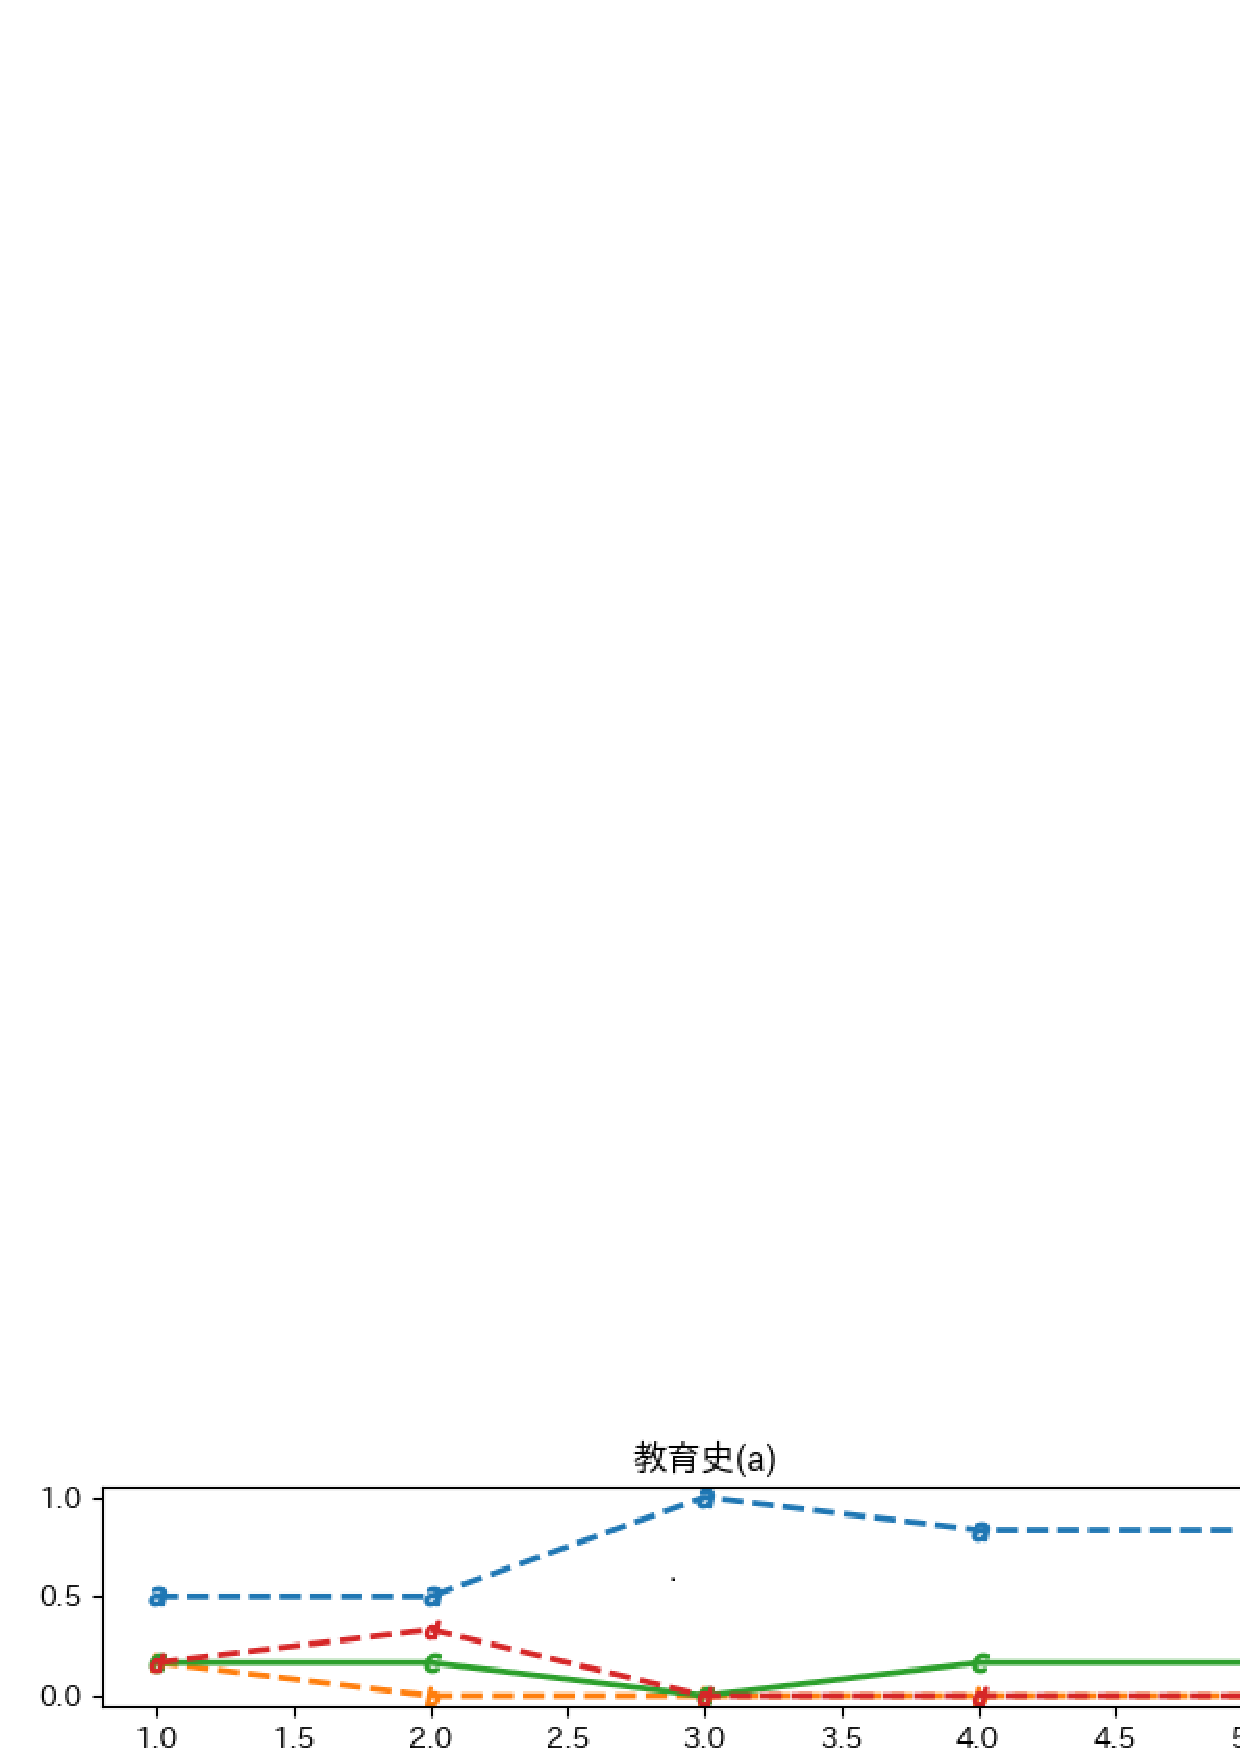
\includegraphics[bb = -50 60 1 1,scale = 0.6]{Figure_1.jpg}
  \vspace{1cm}
\end{figure}

\ \ 正答率は中位群までは上昇していて、上位群では多少差はあるが高い正答率を有している。下位識別力項目に近い項目特性図をしている。

$\bigcirc$第$2$問目について、項目特性図は以下の通りになった。
\vspace{1cm}
\begin{figure}[H]
  \includegraphics[bb = -50 60 1 1,scale = 0.6]{Figure_2.jpg}
\end{figure}
\leavevmode \\
\\
\ \ 下位群から中位群までは正答率は低いが、そこから上位群にかけて急激に上昇している。$1$問目より下位識別力項目の項目特性図をしている。

$\bigcirc$第$3$問目について、項目特性図は以下の通りになった。
\vspace{1cm}
\begin{figure}[H]
  \includegraphics[bb = -40 60 1 1,scale = 0.8]{Figure_3.jpg}
\end{figure}
\leavevmode \\
\\
\ \ 下位群から上位群に行くにつれて順当に正答率が上がっている。項目特性図は高識別力項目と言える。

$\bigcirc$第$4$問目について、項目特性図は以下の通りになった。
\vspace{1cm}
\begin{figure}[H]
  \includegraphics[bb = -50 60 1 1,scale = 0.6]{Figure_4.jpg}
\end{figure}
\leavevmode \\
\\
\ \ 正答率はどの群も安定して$6$割を超えて最上位群は正答率が$1$である。項目特性図は高通過率項目に近い。

$\bigcirc$第$5$問目について、項目特性図は以下の通りになった。
\vspace{1cm}
\begin{figure}[H]
  \includegraphics[bb = -50 60 1 1,scale = 0.6]{Figure_5.jpg}
\end{figure}
\leavevmode \\
\\
\ \ 正答率は全体的に高位に張り付いている。$4$問目より高通過率項目である。

$\bigcirc$第$6$問目について、項目特性図は以下の通りになった。
\vspace{1cm}
\begin{figure}[H]
  \includegraphics[bb = -50 60 1 1,scale = 0.6]{Figure_6.jpg}
\end{figure}
\leavevmode \\
\\
\ \ 正答率は下位群から中位群にかけては上昇しており、上位群では安定した正答率を有している。型としては、下位識別力項目である。

$\bigcirc$第$7$問目について、項目特性図は以下の通りになった。
\vspace{1.5cm}
\begin{figure}[H]
  \includegraphics[bb = -50 60 1 1,scale = 0.6]{Figure_7.jpg}
\end{figure}
\leavevmode \\
\\
\ \ $5$問目と似ていて正答率は全体的に高位に張り付いている。高通過率項目である。
\newpage

$\bigcirc$第$8$問目について、項目特性図は以下の通りになった。
\vspace{1.5cm}
\begin{figure}[H]
  \includegraphics[bb = -50 60 1 1,scale = 0.6]{Figure_8.jpg}
\end{figure}
\leavevmode \\
\\
\ \ 下位群から上位群に行くにつれて順当に正答率が上がっている。項目特性図は高識別力項目と言える。
\\

\section{能力値や項目パラメータの推定}
\subsection{最尤推定法}
ここでは項目パラメータが既知の場合に、項目パラメータと反応行列から能力値$\theta$の推定値を求める方法を紹介する。

受験者$i$の能力値$\theta_i$は現実においては未知である。
一方で、反応行列は収集して実際の値として固定し用いることができる。そこで、反応行列を既知として、能力値$\theta_i$を変数として扱うことにする。このとき$p_j(\boldsymbol{u}_i | \theta_i)$に対して、$L(\theta_i|\boldsymbol{u}_{i})$を確率ではなく尤度と呼び、その尤度関数を、
\begin{align}
  \label{01}
  \displaystyle L(\theta_i|\boldsymbol{u}_{i}) =\prod_{j = 1}^{n} p_{j}(\theta_i)^{u_{ij}} (1 - p_{j})(\theta_i)^{1 - u_{ij}}
\end{align}
と定義する。このとき、尤度が最大になるときの項目パラメータの値を、パラメータの推定値として利用する。このような推定法を最尤推定法という。つまり、この推定法は実際のデータが最も得られやすいようなパラメータの値を決める方法である。

また、最尤推定値の性質として以下のことがあげられる。
\begin{itemize}
  \item 受験者$i$の反応ベクトル$\boldsymbol{u_i} = (u_{i1}, u_{i2}, \cdots, u_{ij})$から計算される最尤推定値は同じタイプの母数であっても、一般に$1$母数、$2$母数、$3$母数モデルでそれぞれに値が異なる。項目特性関数が異なるため、尤度関数の形状も異なるので最大値が一致しないのは自然である。
  \item 全問正答、全問誤答の最尤値はそれぞれ$\theta_i = \infty,\theta_i = -\infty$となり事実上は解が求まらない。
\end{itemize}

次に、具体的に式(\ref{01})を最大化する$\hat{\theta_i}$を考える。そこで、式(\ref{01})の対数をとり、
\begin{align}
  \displaystyle \log L(\theta_i | u_{i}) =\sum_{j = 1}^{n} [u_{ij} \  \log \  p_{j}(\theta_i) + (1 - u_{ij}) \ \log \  q_{j}(\theta_i)]
\end{align}
を考える。この関数を対数尤度関数という。この対数尤度関数最大にする$\hat{\theta_i}$を求める解法が考えられる。
\subsection{同時最尤推定法}
前節では、項目パラメータは既知である場合について考えてきた。ここでは、受験者たちの反応行列$\boldsymbol U$から受験者の能力値$\theta$と項目パラメータを同時に推定する方法を考える。受験者$i$の能力値$\theta_i$が与えられたときの$\theta_i$の尤度の分布は
\begin{align}
  \displaystyle
  L(\theta_i,a_j,b_j,c_j|u_{ij}) = p_j(\theta_i)^{u_{ij}} (1 - p_j(\theta_i))^{1 - u_{ij}}
\end{align}のように定義される。ここで項目同士は局所独立を考えている。局所独立とは、項目同士が互いに正答率に影響していない状態のことである。本節では、能力値$\theta$だけではなく、項目パラメータも未知であることを仮定しているので、$\theta_i$の尤度の分布を以下のように書き直す。
\begin{align}
  \displaystyle L(\theta_i,\boldsymbol{a},\boldsymbol{b},\boldsymbol{c}| \boldsymbol{u}_{i}) = \prod_{j = 1}^{n} p_j(\theta_i)^{u_{ij}}(1- p_j(\theta_i))^{1-u_{ij}}
\end{align}
となる。
$3$母数ロジスティックモデルを用いて考える。$n$個の長方形の和によって$L(\theta_i,a_j,b_j,c_j|u_{ij})$の値を近似することができる。
ここで、
\begin{align*}
  \displaystyle \boldsymbol{a}&=(a_1,a_2,\cdots,a_n)^{t} \\
  \boldsymbol{b}&= (b_1,b_2,\cdots,b_n)^{t} \\
  \boldsymbol{c}&= (c_1,c_2,\cdots,c_n)^{t} \\
  \boldsymbol{\theta}&= (\theta_1,\theta_2,\cdots,\theta_N)^{t}
\end{align*}
とし、受験者の反応は互いに独立と考えられることから、能力値$\theta$と項目パラメータが与えられた条件の下で、$n$個の項目に対する$N$人の受験者の反応行列$\boldsymbol{U}$が観察される尤度は、
\begin{align}
  \displaystyle L(\boldsymbol{\theta},\boldsymbol{a},\boldsymbol{b},\boldsymbol{c}| \boldsymbol{U})\nonumber &= \prod_{i = 1}^{N} L(\theta_i,\boldsymbol{a},\boldsymbol{b},\boldsymbol{c}|\boldsymbol{u}_i)\\ &= \prod_{i = 1}^{N}\prod_{j = 1}^{n} L(\theta_i,a_j,b_j,c_j|u_{ij})
\end{align}
と表現される。この尤度を最大にする各項目パラメータの値のベクトルが最尤推定値である。またこのような方法が最尤推定法であった。ここで最大値を求めるために、対数変換を行うと
\begin{align}
  \displaystyle \log L(\boldsymbol{\theta},\boldsymbol{a},\boldsymbol{b},\boldsymbol{c}|\boldsymbol{U})  &= \log \prod_{i = 1}^{N}\prod_{j = 1}^{n} L(\theta_i,a_j,b_j,c_j|u_{ij})\nonumber\\ &=  \log \prod_{i = 1}^{N}\prod_{j = 1}^{n}  p_j(\theta_i)^{u_{ij}}(1- p_j(\theta_i))^{1-u_{ij}} \nonumber \\ &=  \sum_{i = 1}^{N} \sum_{j = 1}^{n} [u_{ij} \log p_j(\theta_i) + (1 - u_{ij}) \log q_j(\theta_i)]
\end{align}
となる。この関数の最大化を考える。尤度関数を最大化するパラメータの値と、対数尤度関数を最大化するパラメータの値は等しい。
対数尤度関数を最大化する解は、変数で微分して$0$とおいた方程式を変数に関して解くことによって求まる。
変数が複数あるので、各変数$\theta_i,a_j,b_j,c_j$で偏微分した結果を$0$とおき、
\begin{align}
  \displaystyle \dfrac{\partial }{\partial \theta_i} \log L(\boldsymbol{\theta},\boldsymbol{a},\boldsymbol{b},\boldsymbol{c}|\boldsymbol{U}) &= \dfrac{\partial }{\partial \theta_i} \sum_{i = 1}^{N} \sum_{j = 1}^{n} [u_{ij} \log p_j(\theta_i) + (1 - u_{ij})\log (1 - p_j(\theta_i))]\nonumber \\ &= D\sum_{j = 1}^{n} \{u_{ij}\{(p_j(\theta_i)- c_j)\frac{-a_j\exp(a_j(\theta_i - b_j))}{1 + c_j \exp(a_j(\theta_i - b_j))}\} \nonumber \\ &+ (1 - u_{ij})\frac{a_j(p_j(\theta_i) - c_j)}{c_j\exp(a_j(\theta_i - b_j))}\}
  \nonumber \\ &=  D\sum_{j = 1}^{n} \frac{a_j(p_j(\theta_i) - c_j)(u_{ij} - p_j(\theta_i))}{(1 - c_j)p_j(\theta_i)}=0     \\
  \displaystyle \dfrac{\partial }{\partial a_j} \log L(\boldsymbol{\theta},\boldsymbol{a},\boldsymbol{b},\boldsymbol{c}|\boldsymbol{U}) &= \frac{D}{1 - c_j}\sum_{i = 1}^{N} \frac{(\theta_i - b_j)(p_j(\theta_i) - c_j)(u_{ij} - p_j(\theta_i))}{p_j(\theta_i)}=0    \\
  \displaystyle \dfrac{\partial }{\partial b_j} \log L(\boldsymbol{\theta},\boldsymbol{a},\boldsymbol{b},\boldsymbol{c}|\boldsymbol{U}) &= \frac{-Da_j}{1 - c_j}\sum_{i = 1}^{N} \frac{(p_j(\theta_i) - c_j)(u_{ij} - p_j(\theta_i))}{p_j(\theta_i)}=0    \\
  \displaystyle \dfrac{\partial }{\partial c_j} \log L(\boldsymbol{\theta},\boldsymbol{a},\boldsymbol{b},\boldsymbol{c}|\boldsymbol{U}) &= \frac{1}{1 - c_j}\sum_{i = 1}^{N} \frac{(u_{ij} - p_j(\theta_i))}{p_j(\theta_i)}=0
\end{align}
上記の式の連立方程式を解いた値が最尤推定値となる。この方法は能力値$\theta$と項目パラメータを同時に推定するという意味で特に同時最尤推定法と呼ぶ。
%参考文献
\subsection{周辺最尤推定法}
同時最尤推定法では、尤度関数を微分した式が多くなってしまうという欠点がある。最大化する尤度関数の中から、能力値$\theta$を消去することができれば、最大化に関するパラメータを大幅に減らすことができる。また受験者を追加してデータを増やしても未知数が増えることはないので推定値が安定するというメリットもある。つまり、反応行列が与えられたときの項目パラメータだけの尤度関数を構成すればよい。この考えを周辺最尤推定法と呼ぶ。

受験者の能力値$\theta$を尤度関数から消去すし項目パラメータを推定する方法を考える。豊田秀樹(2012)から引用して説明する。
例中では、説明変数は離散型として$4$つの値$\displaystyle \theta = 1.0,0.5,-0.5,-1.0$しかとらないと仮定する。例えば、それらを「優」、「良」、「可」、「不可」とみなしそのような学生が大学の中に$0.3,0.2,0.2,0.3$の確率で存在しているものとする。このとき、母集団から受験者を選び出し、反応ベクトル$\boldsymbol{u}_i$を得る。$L(\theta_i,\boldsymbol{a,b,c}|\boldsymbol{u}_i)$の能力値$\theta_i$に具体的な尺度値を代入して、$g(\theta_i)$との積和を求める。式は、
\begin{align}
  \begin{split}
  \displaystyle L(\theta,\boldsymbol{a,b,c}\boldsymbol{u}_i) &= g(1.0)L(1.0,\boldsymbol{a,b,c}|\boldsymbol{u}_i) + g(0.5)L(0.5,\boldsymbol{a,b,c}|\boldsymbol{u}_i)\\&\quad + g(-0.5)L(-0.5,\boldsymbol{a,b,c}|\boldsymbol{u}_i) + g(-1.0)L(-1.0,\boldsymbol{a,b,c}|\boldsymbol{u}_i)\\ &= 0.3L(1.0,\boldsymbol{a,b,c}|\boldsymbol{u}_i) + 0.2L(0.5,\boldsymbol{a,b,c}|\boldsymbol{u}_i)\\&\quad + 0.2L(-0.5,\boldsymbol{a,b,c}|\boldsymbol{u}_i) + 0.3L(-1.0,\boldsymbol{a,b,c}|\boldsymbol{u}_i)
  \end{split}
\end{align}
のように導く。このように局外パラメータを確率分布から消去するために局外パラメータの分布と局外パラメータで条件つけられた確率分布との積和を計算することで能力値$\theta_i$を消去することができた。このことを、周辺化による局外パラメータの消去という。

能力値の階級の幅を狭めることができれば実質離散型として扱うことができる。例えば、小学$1$年生の体重を記録する際に、$10$kgから$35$kgまでを$0.2$kg刻みの離散変数として扱うことができる。そこで、$K$個の値をとる階級値$\displaystyle \theta_k$の分布$\displaystyle g(\theta_k)$を考える。これを、多項分布という。添え字$k$は受験者ではなくヒストグラムの階級値についていることに注意する。このとき、母集団から$1$人の受験者を抽出し受験させ$\displaystyle \boldsymbol{u}_i$という結果を得る尤度は、
\begin{align}
  \displaystyle  L(\boldsymbol{a,b,c}|\boldsymbol{u}_i) = \sum_{k = 1}^{K} g(\theta_k)L(\theta_k,\boldsymbol{a,b,c}| \boldsymbol{u}_i)
\end{align}
と表現され、能力値$\theta$は消去される。ただしこの場合は能力値$\theta$の母集団におけるヒストグラムが既知であることが必要である。
\subsection{ベイズ推定法}
最尤推定法では、全問正答全問誤答の場合は、推定することができなかった。項目パラメータの分布を利用した推定方法に、ベイズ推定法がある。これは、全問正答、誤答の尺度値を推定することができる。まずは、ベイズの定理から説明する。
\subsubsection{ベイズの定理}
  ある確率事象を$A$、$B$とする。$P(B)$は事象$B$が起こる確率であり。$P(A|B)$は事象$B$が起こる仮定の上で、事象$A$が起こる確率とする。二つの積は、積事象の確率とし$P(A \cap B)$とする。これらの関係を式にすると、
  \begin{align}
    \label{000}
    \displaystyle P(A \cap B) = P(B)P(A|B)
  \end{align}
  となる。両辺を$P(B)$で割ると、
  \begin{align}
    \label{001}
    \displaystyle P(A|B) = \frac{P(A \cap B)}{P(B)}
  \end{align}
  となる。ここで$A$と$B$は一般的な事象を表しているので、式(\ref{000})の$A$と$B$を入れ替えると、
  \begin{align}
    \displaystyle P(A \cap B) = P(A)P(B|A)
    \end{align}
  である。これを式(\ref{001})に代入すると、
  \begin{align}
    \label{003}
    \displaystyle P(A|B) = \frac{P(A)P(B|A)}{P(B)}
  \end{align}
  となり、この式をベイズの定理という。これを項目反応理論に応用するために式を変形していく。式($\ref{003})$を$A$を$H$に、$B$を$D$に置き換える。
  \begin{align}
    \label{0004}
    \displaystyle
    P(H|D) = \frac{P(H)P(D|H)}{P(D)}
  \end{align}
  さらに、標本空間$\Omega$の事象$D$には複数の原因$H_i (i = 1, 2, 3, \cdots, M)$があると仮定する。原因$H_i$について以下のような仮定を考える。
  \begin{itemize}
    \item $\forall i, j $($\hspace{3pt} i \neq j$)について$H_i \cap H_j = \varnothing$
    \item $H_1 \cup H_2  \cup \cdots \cup H_M = \Omega$
  \end{itemize}
  上記の$2$つを二つを仮定すると、事象が起こる確率$P(D)$は以下のような式になる。
  \begin{align}
    \label{0005}
    \displaystyle
    P(D) = P(D \cap H_1) + P(D \cap H_2)  + \cdots + P(D \cap H_M)
  \end{align}
  ここで、$P(D)$は次のように整理することができる。
  \begin{align}
    \label{0006}
    \displaystyle
    P(D) = P(D|H_1)P(H_1) + P(D|H_2)P(H_2) + \cdots + P(D|H_M)P(H_M)
  \end{align}
  式$(\ref{0006})$を式$(\ref{0004})$に代入すると、
  \begin{align}
    \label{0007}
    \displaystyle
    P(H_i|D) &= \frac{P(H_i)P(D|H_i)}{P(D|H_1)P(H_1) + P(D|H_2)P(H_2) + \cdots + P(D|H_M)P(H_M)} \notag \\
    &= \frac{P(D|H_i)P(H_i)}{\displaystyle\sum_{i = 1}^M P(D|H_i)P(H_i)}
  \end{align}
  となる。
  ここで$P(H_i|D)$は事後確率、$P(H_i)$を事前確率という。さらに、$P(D|H_i)$は原因$H_i$の下で結果$D$が得られる確率を意味し尤度という。
  %また、$P(D|H_i)$を$P(\boldsymbol{u}_i | \theta_i)$とし、$P(H_i)$を$\pi(\theta_i)$とすると以下のような式になる。
  %\begin{align}
  % \label{0009}
  %  \displaystyle
  %  p(\theta_i|\boldsymbol{u}_i) = \frac{p(\boldsymbol{u}_i | \theta_i)\pi(\boldsymbol{u}_i)}{\displaystyle \int_{-\infty}^{+\infty} p(\boldsymbol{u}_i | \theta_i)\pi(\boldsymbol{u}_i) d\theta_i}
  %\end{align}
\subsubsection{EAP法(Expected a posteriori法)}
次にEAP法を紹介する。これは、$\theta_i$の事後分布の密度関数の$\theta_i$に関する平均値を推定値とする推定法である。これは、2乗損失もとでは事後分布の平均が2乗損失を最小にするという事実に基づいた推定法である。式にすると、
\begin{align}
  \displaystyle
  E[\theta_i | \boldsymbol{u}_i] = \int_{-\infty}^{+\infty} \theta_i \frac{p(\boldsymbol{u}_i | \theta_i)\pi(\theta_i)}{\displaystyle \int_{-\infty}^{+\infty} p(\boldsymbol{u}_i | \theta_i)\pi(\theta_i) d\theta_i} d\theta_i =  \frac{\displaystyle\int_{-\infty}^{+\infty} \theta_i \pi(\theta_i)p(\boldsymbol{u}_i|\theta) d\theta_i}{\displaystyle\int_{-\infty}^{+\infty}  \pi(\theta_i)p(\boldsymbol{u}_i|\theta) d\theta_i}
\end{align}
となる。ただし、$\pi(\theta)$は$\theta$の事前分布の密度関数である。式中の積分は区分求積法によって求めることができる。

ある区間$[a,b]$を$M$等分した点$(幅は\Delta \theta)$を$\theta_m(m = 1,2,\cdots ,M,M+1)$とすると
\begin{align}
  \displaystyle \int_{b}^{a} f(\theta) d\theta \simeq \sum_{m=1}^{M} f(\theta) \times \Delta \theta
\end{align}
によって左辺を$N$個の長方形の面積の和に近似することができる。式$(3.5)$中の区間は$[-\infty,\infty]$であるが、$\pi(\theta)$は標準正規分布の密度関数を仮定しているので、積分区間は$[-3,3]$や$[-4,4]$などで十分であると考えられる。式にすると、
\begin{align}
  \displaystyle \hat{\theta}_i \simeq \frac{\displaystyle\sum_{m=1}^{M} \theta_{m} p(\boldsymbol{u}_i | \theta_{m})\pi(\theta_{m})\Delta \theta}{\displaystyle\sum_{m=1}^{M} p(\boldsymbol{u}_i | \theta_{m})\pi(\theta_{m})\Delta \theta}
\end{align}
と近似できる。
これを、能力値$\theta$だけでなく、項目パラメータに用いることで推定値を求めることができる。
そのためには、項目パラメータの事前分布を仮定しておく必要がある。
\begin{description}[labelwidth=10em]
  \item[能力値$\theta$の事前分布] 能力値$\theta$の事前分布には正規分布が仮定されることが多い。正規分布のパラメータは平均$\mu_\theta$と分散${\sigma}^2 _\theta$である。
  \item[識別力$a$の事前分布] 識別力の推定値は数学的には負の値もとり得るが、識別力の事前分布には正の範囲で定義される対数正規分布が仮定されることが多い。
  \item[困難度$b$の事前分布] 困難度の事前分布にも正規分布が仮定されることが多い。
  \item[偶然率$c$の事前分布] 偶然率の推定値は確率を表現するパラメータである。このため事前分布はベータ分布が仮定されることが多い。ベータ分布のパラメータは$\alpha,\beta$であり、密度関数は
  \begin{align}
    \displaystyle
    \frac{x^{\alpha - 1} (1 - x)^{\beta - 1}\Gamma(\alpha + \beta)}{\Gamma(\alpha) \Gamma(\beta)}
  \end{align}
  ベータ分布の最頻値は、
  \begin{align}
    \displaystyle
    \frac{\alpha - 1}{\alpha + \beta- 2}
  \end{align}
  であることが知られている。選択形式の問題の場合、偶然率の尤もらしい目安は選択肢数$k$の逆数$\frac{1}{k}$と考えられる。目安$\frac{1}{k}$を事前分布の最頻値の一致させるならば、例えば、
  \begin{align}
    \displaystyle
    \alpha = 20 \times \frac{1}{k} + 1\\
    \beta = 20 \times (1 - \frac{1}{k}) + 1
  \end{align}
  とする。$5$肢選択ならば$c = 0.2$とし$\alpha = 5,\beta = 17$のベータ分布を考える。
\end{description}

\subsection{推定値と考察}
\subsubsection{ベイズ推定}
第$2$章のテストの反応行列を用いてベイズ推定法で項目パラメータと能力値$\theta$を推定する。
\[ \boldsymbol{U} =
\left(
\renewcommand{\arraycolsep}{3pt}
\begin{array}{cccccccccccccccccccccccccccccc}
1 & 0 & 0 & 0 & 1 & 0 & 0 & 1 & 0 & 1 & 0 & 0 & 0 & 0 & 0 & 0 & 0 & 1 & 0 & 0 & 0 & 0 & 1 & 1 & 1 & 1 & 0 & 0 & 1 & 1\\
0 & 0 & 0 & 0 & 1 & 0 & 0 & 1 & 0 & 0 & 0 & 0 & 0 & 0 & 0 & 0 & 0 & 0 & 1 & 1 & 0 & 0 & 0 & 0 & 0 & 0 & 1 & 0 & 0 & 0\\
0 & 0 & 0 & 1 & 0 & 0 & 0 & 0 & 0 & 0 & 0 & 0 & 0 & 0 & 1 & 0 & 0 & 0 & 0 & 0 & 1 & 1 & 0 & 0 & 0 & 0 & 0 & 0 & 0 & 0\\
1 & 0 & 1 & 0 & 0 & 0 & 0 & 1 & 1 & 0 & 0 & 0 & 0 & 0 & 0 & 0 & 0 & 0 & 0 & 0 & 0 & 0 & 0 & 0 & 0 & 0 & 0 & 0 & 0 & 0\\
0 & 0 & 1 & 0 & 0 & 0 & 1 & 0 & 0 & 0 & 1 & 0 & 0 & 0 & 1 & 0 & 0 & 0 & 1 & 0 & 0 & 0 & 0 & 0 & 0 & 0 & 1 & 0 & 0 & 0\\
0 & 0 & 0 & 1 & 0 & 0 & 1 & 0 & 0 & 0 & 0 & 0 & 1 & 0 & 0 & 0 & 1 & 0 & 0 & 0 & 1 & 0 & 0 & 0 & 0 & 0 & 0 & 0 & 1 & 0\\
1 & 0 & 0 & 0 & 1 & 0 & 0 & 0 & 1 & 0 & 0 & 0 & 1 & 0 & 0 & 0 & 1 & 1 & 0 & 0 & 1 & 0 & 1 & 0 & 1 & 1 & 0 & 0 & 1 & 0\\
0 & 0 & 1 & 0 & 0 & 0 & 1 & 0 & 0 & 0 & 1 & 0 & 0 & 0 & 1 & 0 & 0 & 1 & 1 & 0 & 0 & 0 & 1 & 0 & 1 & 1 & 1 & 0 & 0 &0
\end{array}
\right)^t
\]
ただし、人数$\times$問題の大きさの行列を使うために実際の計算には行列を転置したものを用いる。
$2$パラメータロジスティックモデルと$3$パラメータロジスティックモデルを用いて推定する。使用するプログラムは付録に掲載する。それぞれのパラメータの推定値は以下のようになった。
\begin{table}[H]
  \begin{minipage}[t]{.45\textwidth}
    \begin{center}
      \begin{tabular}{|l||c|c|} \hline
        & 困難度& 識別力 \\ \hline \hline
        $問題1$ & $0.329$ & $0.369$  \\ \hline
        $問題2$ & $0.767$ & $0.843$  \\ \hline
        $問題3$ & $1.091$ & $0.705$   \\ \hline
        $問題4$ & $1.019$ & $0.766$   \\ \hline
        $問題5$ & $0.197$ & $3.083$   \\ \hline
        $問題6$ & $0.958$ & $0.534$   \\ \hline
        $問題7$ & $0.259$ & $0.431$   \\ \hline
        $問題8$ & $-0.18$ & $3.212$   \\ \hline
      \end{tabular}
    \end{center}
    \caption{$2$パラメータロジスティックモデル}
  \end{minipage}
  \begin{minipage}[t]{.45\textwidth}
    \vspace{-2.83cm}
    \begin{center}
      \begin{tabular}{|l||c|c|c|} \hline
        & 困難度& 識別力 & 偶然率\\ \hline \hline
        $問題1$ & $1.414$ & $1.622$ &$0.350$ \\ \hline
        $問題2$ & $0.958$ & $1.674$ &$0.140$ \\ \hline
        $問題3$ & $1.275$ & $1.787$ &$0.137$ \\ \hline
        $問題4$ & $1.274$ & $1.785$ &$0.136$ \\ \hline
        $問題5$ & $0.026$ & $2.970$ &$0.038$ \\ \hline
        $問題6$ & $1.334$ & $1.779$ &$0.200$ \\ \hline
        $問題7$ & $1.414$ & $1.623$ &$0.350$ \\ \hline
        $問題8$ & $-0.487$ & $3.175$ &$0.044$ \\ \hline
      \end{tabular}
    \end{center}
    \caption{$3$パラメータロジスティックモデル}
  \end{minipage}
\end{table}
困難度の推定値に関して、$2$パラメータロジスティックモデルと$3$パラメータロジスティックモデルを比べると$2$パラメータロジスティックモデルよりも$3$パラメータロジスティックモデルの結果の方が最大値と最小値の差が$2$パラメータロジスティックモデルでは$1.271$、$3$パラメータロジスティックモデルでは$1.901$と広がっている。つまり、$2$パラメータロジスティックモデルで推定して難しいと推定された項目は$3$パラメータロジスティックモデルではより難しいと判断され、簡単と推定された問題はより簡単と推定される結果となった。これは偶然率がパラメータに入ったことで、難しい問題は実力で正解することがより難しくなっていることに起因していると考えられる。
\vspace{4cm}
\begin{figure}[H]
  \centering
  \includegraphics[bb = 1000 100 1 1,scale = 0.3]{maxmin.png}
  \vspace{1cm}
  \caption{困難度の推定値}
\end{figure}
\begin{itemize}
  \item[]
  \item[] また、他にも以下のようなことが分かる。
  \item[1] 第$5$問と第$8$問がともに高い値が出ている。第$5$問と第$8$問はともに偶然率が低く偶然正解することが少ないことを考えるとほとんどの受験者が実力通りの結果が出ていて能力値$\theta$をしっかり測れる項目である。
  \item[2] 第$4$問と第$5$問に関しては同じ高通過率項目、つまり多くの受験者が正解している項目であるが困難度は第$4$問の方が高く、識別力は第$5$問の方が高い。さらに、項目特性図を比べると第$5$問の方が正答率がより高位に張り付いた状態になっていて、第$4$問は誤答も万遍なくある状態になっている。つまり、第$4$問の方がしっかりと選択肢が機能していて「良い」問題といえる。
  \item[]
\end{itemize}
また図$7$は、能力値$\theta$の推定値をグラフ化したものである。困難度がより高く推定された$3$パラメータロジスティックモデルの能力値$\theta$の推定値のほうが、$2$パラメータロジスティックモデルの能力値$\theta$の推定値より、低く推定されている。
ここで、能力値$\theta$の推定値を標準化しその値を用いて、グラフに表すと、図$8$のようになった。
\vspace{3cm}
\begin{figure}[H]
  \centering
  \includegraphics[bb = 550 100 1 1,scale = 0.7]{maxmin_theta.png}
  \vspace{2cm}
  \caption{能力値$\theta$の推定値}
\end{figure}
\vspace{4cm}
\begin{figure}[H]
  \centering
  \includegraphics[bb = 550 100 1 1,scale = 0.7]{bay2bay3.png}
  \vspace{2cm}
  \caption{能力値$\theta$の推定値(標準化ver)}
\end{figure}
また、能力値$\theta$の推定値については以下のようなことがわかる。
\begin{itemize}
  \item[1] 標準化すると$2$パラメータも$3$パラメータも似たような値を推定している。
  \item[2] 受験者$7$と受験者$8$や、受験者$22$と受験者$23$の関係のように$2$パラメータも$3$パラメータで能力値$\theta$の大小関係が逆転している箇所が見られる。
  \item[$\rightarrow$] 各受験者の正誤を表した反応ベクトルを調べると受験者$7$と受験者$8$について、総合得点($8$問中$3$問正解)は同じであるが、偶然率の値が高い問題$1$に受験者$7$は誤答、受験者$8$は正答している。また、偶然率の値が低い問題$5, 8$に受験者$7$は正答、受験者$8$は誤答している。これらのことから$2$パラメータで推定したとき、$2$人の受験者はしっかり実力で$3$問正解しているため、困難度が高い問題により正解している受験者$7$の方が受験者$8$よりも高い評価を受けているが、偶然率を踏まえると、より実力で正解している受験者$8$の方が評価されている
\end{itemize}
\subsubsection{最尤推定法との比較}
ここで、最尤推定法も用いた推定値との比較もしていく。まずは、最尤推定法を用いた推定値とベイズ推定法の値($2$パラメータ)を表にまとめたものと能力値$\theta$を標準化しグラフに表したものを以下に示す。
\begin{table}[H]
  \begin{minipage}[t]{.45\textwidth}
    \begin{center}
      \begin{tabular}{|l||c|c|} \hline
        & 困難度& 識別力 \\ \hline \hline
        $問題1$ & $0.329$ & $0.369$  \\ \hline
        $問題2$ & $0.767$ & $0.843$  \\ \hline
        $問題3$ & $1.091$ & $0.705$   \\ \hline
        $問題4$ & $1.019$ & $0.766$   \\ \hline
        $問題5$ & $0.197$ & $3.083$   \\ \hline
        $問題6$ & $0.958$ & $0.534$   \\ \hline
        $問題7$ & $0.259$ & $0.431$   \\ \hline
        $問題8$ & $-0.18$ & $3.212$   \\ \hline
      \end{tabular}
    \end{center}
    \caption{ベイズ推定法}
  \end{minipage}
  \begin{minipage}[t]{.45\textwidth}
    \vspace{-2.83cm}
    \begin{center}
      \begin{tabular}{|l||c|c|} \hline
        & 困難度& 識別力 \\ \hline \hline
        $問題1$ & $-6.87$ & $0.640$  \\ \hline
        $問題2$ & $-2.87$ & $0.841$  \\ \hline
        $問題3$ & $-0.87$ & $3.999$   \\ \hline
        $問題4$ & $0.461$ & $2.705$   \\ \hline
        $問題5$ & $1.461$ & $1.091$   \\ \hline
        $問題6$ & $2.261$ & $0.671$   \\ \hline
        $問題7$ & $2.928$ & $0.266$   \\ \hline
        $問題8$ & $3.499$ & $0.194$   \\ \hline
      \end{tabular}
    \end{center}
    \caption{最尤推定法}
  \end{minipage}
\end{table}
\vspace{3cm}
\begin{figure}[H]
  \centering
  \includegraphics[bb = 1300 100 1 1,scale = 0.3]{saiyubay.png}
  \vspace{1cm}
  \caption{能力値$\theta$の推定値(標準化ver)}
\end{figure}
全問不正解の受験者がいるので、最尤推定法の性質上、能力値の推定値は$-\infty$になる。グラフは下限を設定しているので、実際は$-2$よりもずっと小さい値を示している。ベイズ推定法と比べても最尤推定法は項目パラメータも安定していないことが分かる。さらに、受験者数も$30$人と少ないため最尤推定法は適していない。
\section{ロジスティックモデルの多次元化}
\setcounter{subsection}{1}
これまで考えてきたモデルは項目が受験者の単一の能力値を測定している仮定が置かれていた。仮に項目が潜在能力値を$2$つ以上測定しているという仮定が成り立つならば、前章までで考えてきたロジスティックモデルの能力値$\theta$を多次元で表現したロジスティックモデルを考えることができる。例えば、数学ならば、「計算力」と「論理力」の$2$つの能力が考えられる。実際のテストの運用ではこのような状況が十分に考えられる。そこで、多次元ロジスティックモデルを考えていく。初めに、一般に知られている多次元ロジスティックモデルを紹介する。
\begin{description}
  \item[多次元ロジスティックモデル] 今回考える多次元ロジスティックモデルは$2$パラメータロジスティックモデルを多次元の能力値のケースへ一般化したものである。$2$パラメータ多次元ロジスティックモデルは次のように表現される。
  \begin{align}
    \displaystyle
    \label{4.1}
    p_j(\theta) = \frac{1}{1 + \exp(-\boldsymbol{{a}_j}^t \boldsymbol{\theta}_i + b_j)}
  \end{align}
  ここで$\boldsymbol{a}$は項目ごとの識別力を表すベクトルである。また、$\boldsymbol{\theta}$も受験者ごとの多次元の能力値を並べたベクトルである。つまり式中の$\boldsymbol{a}_j \boldsymbol{\theta_i} + b_j$は次のように表現することができる。
  \begin{align}
    \displaystyle
    \boldsymbol{{a}_j}^t \boldsymbol{\theta_i} + b_j = \sum_{l = 1}^{L} {a_{jl}}\theta_{il} + b_j
  \end{align}
  能力が$2$次元なものであると仮定して考えると
\begin{align}
  \displaystyle
  \boldsymbol{\theta} = (\theta_1,\theta_2)^t
\end{align}
のように項目が受験者の違う$2$つ能力値を測定していると仮定する。しかし、$2$次元で考えるがゆえの問題も出てくる。$2$つの能力値のうちどちらか$1$つの能力値を推定するための基準となる問題が必要になる。問題の識別力ベクトルの向きが決まっていないと、推定したい能力値が正確に測れていないのではないかと考えられる。また、$2$つの識別力ベクトルは一次独立のものを仮定することで$1$次元の話と区別するようにする。前章までに使用した各パラメータの事後密度の期待値を用いたベイズ推定法を使用して能力値や項目パラメータを推定する。
\end{description}
\section{多次元ロジスティックモデルを用いた能力値推定のための問題選定(仮)}
実際にテストを作成する際に問題は作成者が意図を持って採用される。受験者の能力を正確に推定しようとするならば、過去に実施していて、項目パラメータが既知である問題ばかりそろえれば能力値の推定値は安定しそうである。しかし、すべて過去に実施されたテストと同じ問題では、内容は全く理解できていないが過去問題を暗記しただけの人は、能力値が高く推定されてしまう。このようなことを防ぐためには、すべて過去問題と同じ問題というわけにもいかない。そこで考えるのは、過去問題もある程度入れつつ、新しい問題も採用するテスト作成である。そのとき過去問題は
\begin{itemize}
  \item 識別力が高いものを選ぶべきなのか
  \item 困難度が高いものを選ぶべきなのか
  \item 過去問題は全体の中でどのくらいの割合で入れるべきなのか
\end{itemize}
などを考えなければならない。

ここで受験者の能力値を測るのは、新しく採用された問題だけでよいのかを考える。前章にある通り、数学における「計算力」と「論理力」の$2$つの能力が項目から測定されると考えると、その$2$つの能力が測れているとする基準となる項目が必要になると考えられる。例えば、過去問題の中で「計算力」「論理力」の$2$つの能力を測定できた問題$20$問と新しく採用された項目パラメータが未知である問題$30$問でテストを作る。まず、
\begin{itemize}
  \item[(1)] 過去問題から新しく採用された問題が$2$つの能力をどのくらい測れているのかなどの項目パラメータを推定する。
  \item[(2)] 新しい問題だけを用いて受験者の能力値を推定する。
\end{itemize}
という流れである。このように過去問題はあくまでも受験者の能力値を推定するための問題の項目パラメータを推定するために使うことで、毎回同じ問題を使わなくても新しい問題で受験者の能力値が測れるのではないかと考える。

この章では、計算機を使って項目パラメータが既知である問題をどのくらいの割合で入れると受験者の能力値が安定するのかをシミュレーションしていく。状況設定は$100$人の受験者に$100$問の問題を解いてもらう。そのうち、一定の割合で項目パラメータが既知である問題を入れる。今回は過去問題が$25$問、$50$問、$75$問の$3$パターンで計算していく。計算の流れとしては、
\begin{itemize}
  \item[1] 過去問題と反応行列から新しい問題の項目パラメータを推定
  \item[2] 項目パラメータが推定された新しい問題を使って受験者の能力値を推定
\end{itemize}
の$2$段階に分ける。ここで以下の$2$点に注意されたい。
\begin{itemize}
  \item 過去問題のパラメータは既知扱いであるので、推定の対象外である。
  \item 受験者の能力値の推定には過去問題は使用せず、新しい問題だけを使用する。
\end{itemize}ここで、各項目パラメータに関しては以下のように設定した。
\begin{itemize}
  \item 識別力は$a_1$と$a_2$とし$2$つのベクトルを考える。$a_1$と$a_2$はそれぞれ別の能力を測っていると考えるために、一次独立な$2$つのベクトルを仮定する。今回は$a_1$は最小値を$0.5$、最大値を$2$とし均等な間隔で$50$個並べ、それを$2$つ繋げたベクトルとし、$a_2$は最大値を$1$とし$a_1$と同じ並べ方をしたベクトルとした。

  $\boldsymbol{a_1} = (0.5, 0.53061, 0.56122, \cdots, 2, 0.5, 0.53061, 0.56122, \cdots, 2)$

  $\boldsymbol{a_2} = (0.5, 0.53061, 0.56122, \cdots, 1, 0.5, 0.53061, 0.56122, \cdots, 1)$
  \item 困難度$b$は最小値$-1$、最大値$1$とし$100$問分間隔が均等になるように並べたベクトルとした。

  $\boldsymbol{b} = (-1, -0.9797, -0.9595, \cdots, 1)$
  \item 能力値$\theta$の設定値は識別力と同じく$\theta_1$と$\theta_2$とし$2$つのベクトルが一次独立になるように設定する。一つは最小値$-2$、最大値$2$とし昇順で$100$人分均等に並べ、他方は最初の$50$人は$-1$、残り$50$人は$1$として並べた。

  $\boldsymbol{\theta_1} = (-2, -1.9595, -1.9191, \cdots, 2)$

  $\boldsymbol{\theta_2} = (-1, -1, -1, \cdots, -1, 1, 1, \cdots, 1)$
\end{itemize}
これらを用いて擬似的な反応行列を生成する。過去問を$100$問中$25$問採用する場合を例に上げ具体的な計算の流れを説明する。
\begin{itemize}
  \item[$(1)$] 新しい問題の項目パラメータを推定する。実際には、$1$回の計算で出てきた推定値を初期値として更新する際に、過去問題の$25$問のパラメータは更新せず、設定値のままにしておき、新しい問題だけの項目パラメータだけを更新する。そして、更新された初期値を用いて$2$回目の計算を行う。その際も過去問題の項目パラメータは更新しない。それによって、新しい問題だけの項目パラメータを推定する。
  \item[$(2)$] 新しい問題の項目パラメータが決定したら、その問題を用いて受験者の能力値を推定する。
  \item[$(3)$]上$2$つの計算を$100$回行い推定値が一定の誤差に収まるように収束するまで計算を続ける。
  \item[$(4)$] 推定値の信頼度を上げるためにこの試行を$100$回行い、それぞれの値の平均値を求める。
\end{itemize}
次の節で実際に行った結果と考察を述べる。
\subsection{項目パラメータと能力値の推定値}
以下に示すのは、能力値$\theta_1$、$\theta_2$の推定値と設定値との誤差の平均を、過去問題の割合毎にまとめたものである。
\begin{table}[H]
  \begin{center}
    \begin{tabular}{|c||c|c|c|c|} \hline
      & 過去問題$0$問& 過去問題$25$問 & 過去問題$50$問 & 過去問題$75$問\\ \hline \hline
      $\theta_1$ & $0.397705342$	& $0.408443905$	& $0.416983791$	& $0.520276119$ \\ \hline
      $\theta_2$ & $0.488909176$	& $0.459919565$	& $0.5123526$	& $0.51364787$ \\ \hline
    \end{tabular}
  \end{center}
\end{table}
推定値に関して以下のようなことがわかった。
\begin{itemize}
  \item 能力値$\theta_1$の推定値に関しては過去問を全く入れなかった場合が設定値との誤差が一番小さくなった
  \item 能力値$\theta_2$の推定値に関しては過去問題を$100$問中$25$問採用した場合が、一番設定値との誤差が少なくなった。
  \item $\theta_1$に関しての過去問題$0$問と過去問題$25$問の差は$0.01$、そして、$\theta_2$に関しての過去問題$0$問と過去問題$25$問の差は$0.03$となっている。
\end{itemize}
上記のことより以下のことが考察できる。
\begin{itemize}
  \item[$\triangle$] 能力値を推定する際には、過去問題は使用せず、新しい問題だけ使用するので、過去問$25$問だと能力値を推定する問題が$75$問と多く推定値が安定したと考えられる。
  \item[$\triangle$] 今回既知として扱った問題は識別力の値が高いものから選んでいるため、過去問題が$50$問や、$75$問だと識別力の値が低い値などを含んでしまうため推定値の精度が下がってしまったと考えられる。逆に過去問題を$25$問だけ既知とすると識別力の値が低くても$1.234$あるので推定値の精度も他に比べて上がったと考えられる。
\end{itemize}
項目パラメータに関して、推定している個数がそれぞれで違うので一概には比較できない。そこで、$1$問目から$25$問目までの推定値の平均を比較してみる。
\begin{table}[H]
  \begin{center}
    \begin{tabular}{|c||c|c|c|c|} \hline
      & 過去問題$0$問& 過去問題$25$問 & 過去問題$50$問 & 過去問題$75$問\\ \hline \hline
      $a_1$ & $0.357032998$	& $0.365192399$	& $0.575955796$	& $0.897635541$
      \\ \hline
      $a_2$ & $0.581752051$	& $0.459429589$	& $0.660244633$	& $0.877362495$
      \\ \hline
      $b$ & $0.200210509$	& $0.256411709$	& $0.308571305$	& $0.547870155$
      \\ \hline
    \end{tabular}
  \end{center}
\end{table}
\begin{itemize}
  \item 項目パラメータ$a_1$に関して、差は$0.01$程、過去問題$0$問の方が過去問題$25$問の方が、小さくなっている。同じように、$a_2$では$0.13$程過去問題$25$問が小さく、$b$は$0.5$ほど過去問題を入れない方が小さくなっている。以上のことから人数が$100$人と少ないため項目パラメータ、特に識別力の値は安定しないと考えられる。
\end{itemize}
\section{最後に}
最後の推定のシミュレーションに関して、今回は項目パラメータの値が高い順に採用した。項目パラメータが既知の問題の取り方は他にも、低い方から取ったり平均が$0$になるように取ったりとパターンはあるので次の機会ではこれらのパターンも試したい。

本章で紹介している通り、付録にR言語を用いたスクリプトを掲載してある。読者自身がテストを運用していく際に、ぜひ使用して分析、評価していただきたい。

本研究を進めるにあたり、岩佐学准教授には指導教員として終始熱心なご指導をいただきました。心から感謝いたします。お礼申し上げます。

\section*{参考文献}
\addcontentsline{toc}{section}{参考文献}
\begin{itemize}
  \item 豊田秀樹(2012).\hspace{3pt}項目反応理論[入門編]
  \item 住 政二郎(2015).\hspace{3pt}適応型テストへの応用―ベイズ EAP 推定法とフィッシャー情報量の概説―
  \item 前川眞一.\hspace{3pt}項目反応理論概説
\end{itemize}
\section*{付録1\hspace{3pt}第$2$章で使用した問題}
\addcontentsline{toc}{section}{付録1\hspace{3pt}第$2$章で使用した問題}
\begin{itemize}
  \item[($1$)]次の文と関係の深い人物を記号で答えてください。アメリカの教育学者。プラグマティズムの立場から生産活動を基礎とする労作学校を主張・実施した。
\end{itemize}
\begin{center}
  (a)デューイ \ (b)フレーベル \ (c)シュプランガー \ (d)スペンサー
%スペンサー、フレーベル、デューイ、シュプランガー
\end{center}
\begin{itemize}
  \item[($2$)]次の文と関係の深い人物を記号で答えてください。従来の「臨画帳」を写すだけの美術教育に反対し、自由画中心の教育を提唱した。
\end{itemize}
\begin{center}
  (a)木下竹次 \ (b)芦田恵之介 \ (c)鈴木三重吉 \ (d)山本鼎
%スペンサー、フレーベル、デューイ、シュプランガー
\end{center}
\begin{itemize}
  \item[($3$)]次の文で間違っているものを答えてください。
    \begin{itemize}
    \item[(a)]特別支援学校の設置義務は都道府県にある。
    \item[(b)]児童福祉司は、児童相談所長の命を受けて、児童の保護その他児童福祉に関する事項について相談に応じ、専門技術に基づき必要な指導を行う等児童福祉増進に努めるものとされている。
    \item[(c)]アメリカの教育学者で近代教授学の父であるとされるのがコメニウスであり、彼はその著書「大教授学」においてすべての民衆を対象にした一般教育を構想し、一斉授業も提唱した。
    \item[(d)]いじめが止んでいる状態というのは、その行為が止んでいる状態が少なくとも$3$カ月継続していることをいう。
    \end{itemize}
\end{itemize}
\begin{itemize}
  \item[($4$)]次の選択肢の中から正しいものを答えてください。
  \begin{itemize}
  \item[(a)]普通免許状は$18$歳未満のもの、高等学校を卒業しないものや禁錮以上の刑に処せられたものにも、条件次第では授与される。
  \item[(b)]教育職員検定は、受験者の人物、学力、実務および身体について、ランダムに選ばれた現職の教員が行う。
  \item[(c)]教員免許更新制は、教員として必要な資質を保持できるように、定期的に最新の知識技能を身につけることで社会の尊厳と信頼を得ることを目指すものである。
  \item[(d)]教員はすべて、免許取得$50$年後に免許更新講習を受けその課程を修了しなければ、免許の有効期間を更新できず免許状はその効力を失う。
  %答えは明らか。
  \end{itemize}
\end{itemize}
\begin{itemize}
  \item[($5$)] 次の空欄に当てはまる語句を選びなさい。すべて国民は、法律の定めるところにより、その保護する子女に(\ \ \ \ \ 1 \ \ \ \ )を受けさせる義務を負う。(日本国憲法)
\end{itemize}
\begin{center}
  (a)教育 \ \ \ \ \ (b)義務教育 \ \ \ \ \ (c)普通教育 \ \ \ \ \  (d)特別教育
%普通教育
\end{center}
\begin{itemize}
  \item[($6$)]次の文は何について述べたものか答えてください。
  \item[]人間が健全な発達をするためには人間社会で多様な経験をすることが必要なことを示してくれた。ヴィクトールと名づけられたその子は、会話はほぼ不可能な状態であった。これは、神経言語学で言われるある期間を過ぎてしまったためだといわれている。この子を題材にフランスでは映画化されそのタイトルは当時、映画界を賑わせた。
  %問題文がわかりつらい。
\end{itemize}
\begin{center}
  (a)アヴェロンの野生児 \ \ \ \ \ (b)野生の少年 \\ (c)言語獲得の臨界期 \ \ (d)フィリップピネル
\end{center}
\begin{itemize}
  \item[($7$)]次の文は何について述べたものか答えてください。
  \item[]記憶のまとまりとしての単位
\end{itemize}
\begin{center}
  (a)メモリ \ \ \ \ \ (b)チャンク \ \ \ \ \ (c)ユニット \ \ \ \ \  (d)ミラー
\end{center}
\begin{itemize}
  \item[($8$)]次の文は何について述べたものか答えてください。
  \item[]学習曲線を描いたときに、難易度によって途中で学習の成果が向上しなくなる現象
\end{itemize}
\begin{center}
  (a)スランプ \ \ \ \ \ (b)停滞減少 \ \ \ \ \ (c)負の強化 \ \ \ \ \  (d)プラトー
\end{center}
\section*{付録2\hspace{3pt}推定に使用したプログラム}
\addcontentsline{toc}{section}{付録2\hspace{3pt}推定に使用したプログラム}
\begin{lstlisting}[caption=最尤推定法,label=fuga]
  IRT <- function(data,epsilon) {
    n <- length(data[,1])
    z <- length(data[1,])
    a_0 <- runif(15,min = 0.5,max = 2)
    a_0 <- a_0*(prod(a_0))^(-1 / z)
    b_0 <- c()
    for (d in 1:z){
    bb <- sum(data[,d])/n
    b_0 <- c(b_0,c(bb))
    }
    b_0 <- b_0-mean(b_0)
    theta_0 <- rep(0, n)

    f_theta <- function(a, b) {
    nouryoku <- c()
    for (j in 1:n){
    cut <-c(data[j,])
    P <- function(x) {
    cutt <- 0
    for (i in 1:z){
        if (cut[i]==1) {
            cutt <- cutt + log(1/(1 + exp((-1.7) * a[i] * (x - b[i]))))
            }
        else{
            cutt <- cutt + log(1 - 1/(1 + exp((-1.7) * a[i] * (x - b[i]))))
            }
                }
        return (cutt)
    }
    #par(new = T)
    #curve(P,xlim = c(-4,4),ylim = c(-10,0))
    nouryoku <- c(nouryoku,c(optimize(P,interval = c(-4,4), maximum = TRUE)$maximum))
    }
    return(nouryoku)
    }


    f_sikibetu <- function(theta,b){
    sikibetu <- c()
    for (i in 1:z){
    cut <-c(data[,i])
    P <- function(a) {
    cutt <- 0
    for (j in 1:n){
        if (cut[j]==1) {
            cutt <- cutt + log(1/(1 + exp((-1.7) * a * (theta[j] - b[i]))))
            }
        else{
            cutt <- cutt + log(1 - 1/(1 + exp((-1.7) * a * (theta[j] - b[i]))))
            }
                }
        return (cutt)
    }
    sikibetu <- c(sikibetu,c(optimize(P,interval = c(0,10), maximum = TRUE)$maximum))
    #sikibetu <- sikibetu * (prod(sikibetu))^(-1/z)
    }
    return(sikibetu)
    }

    f_konnando <- function(theta, a) {
    konnando <- c()
    for (i in 1:z){
    cut <-c(data[,i])
    P <- function(b) {
    cutt <- 0
    for (j in 1:n){
        if (cut[j]==1) {
            cutt <- cutt + log(1/(1 + exp((-1.7) * a[i] * (theta[j] - b))))
            }
        else{
            cutt <- cutt + log(1 - 1/(1 + exp((-1.7) * a[i] * (theta[j] - b))))
            }
                }
        return (cutt)
    }
    konnando <- c(konnando,c(optimize(P,interval = c(-2,2), maximum = TRUE)$maximum))
    konnando <- konnando-mean(konnando)
    }
    return(konnando)
    }

    for (i in 1:100){
        theta_1 <- f_theta(a_0,b_0)
        a_1 <- f_sikibetu(theta_1,b_0)
        b_1 <- f_konnando(theta_1,a_1)
        diffrence_theta <- max(abs(theta_1 - theta_0))
        diffrence_a <- max(abs(a_1 - a_0))
        diffrence_b <- max(abs(b_1 - b_0))
        if(diffrence_theta < epsilon & diffrence_a < epsilon & diffrence_b < epsilon){
           print(i)
       break()
        }
        theta_0 <- theta_1
        a_0 <- a_1
        b_0 <- b_1
    }
    return(list(a_0, b_0, theta_0))
    }
  \end{lstlisting}
  \begin{lstlisting}[caption=ベイズ推定法,label=fuge]
    expectation_theta <- function(data, a, b, c) {#nolint
    estimates_theta <- c()
    for (j in 1:dim(data)[1]) {
    cut <- c(data[j, ])
    P <- function(theta) {#nolint
    cutt <- 1
    for (i in 1:50) {
        if (cut[i] == 1) {
            cutt <- cutt * LP3(theta, a[i], b[i], c[i])
            }
        else{
            cutt <- cutt * (1 - LP3(theta, a[i], b[i], c[i]))
            }
                }
        return (cutt)
    }
    cunt_numerator <- 0
    cunt_denominator <- 0
    for (h in 1:41) {
        cunt_numerator <-cunt_numerator+((-4 + (h-1) * 0.2) * P(-4 + (h-1) * 0.2) * prior_distribution_theta(-4 + (h-1) * 0.2) * 0.2) # nolint

        cunt_denominator <- cunt_denominator + (P(-4 + (h-1) * 0.2) * prior_distribution_theta(-4 + (h-1) * 0.2) * 0.2)#nolint
    }
    estimates_theta <- c(estimates_theta, c(cunt_numerator / cunt_denominator))
    }
    return(estimates_theta)
    }

    expectation_a <- function(data, b, theta, c, a) {
    estimates_a <- c()
    for (i in 1:dim(data)[2]) {
    cut <- c(data[, i])
    P <- function(a) {
    cutt <- 1
    for (j in 1:dim(data)[1]) {
        if (cut[j] == 1) {
            cutt <- cutt * (LP3(theta[j], a, b[i], c[i])) #nolint
            }
        else{
            cutt <- cutt * (1 - LP3(theta[j], a, b[i], c[i]))#nolint
            }
                }
        return(cutt)
    }
    cunt_numerator <- 0
    cunt_denominator <- 0
    for (h in 1:40) {
        cunt_numerator <-cunt_numerator+(((h) * 0.1) * P((h) * 0.1) * prior_distribution_a((h) * 0.1) * 0.1) # nolint

        cunt_denominator <- cunt_denominator + (P((h) * 0.1) * prior_distribution_a((h) * 0.1) * 0.1)#nolint
    }
    estimates_a <- c(estimates_a, c(cunt_numerator / cunt_denominator))
    }
    a[1:50] <- estimates_a[1:50]
    return(a)
    }



    expectation_b <- function(data, a, theta, c, b) {
    estimates_b <- c()
    for (i in 1:dim(data)[2]) {
    cut <- c(data[, i])
    P <- function(b) {#nolint
    cutt <- 1
    for (j in 1:dim(data)[1]) {
        if (cut[j] == 1) {
            cutt <- cutt * (LP3(theta[j], a[i], b, c[i]))
            }
        else{
            cutt <- cutt * (1 - LP3(theta[j], a[i], b, c[i]))
            }
                }
        return(cutt)
    }
    cunt_numerator <- 0
    cunt_denominator <- 0
    for (h in 1:40) {
        cunt_numerator <- cunt_numerator + ((-4 + (h-1) * 0.2) * P(-4 + (h-1) * 0.2) * prior_distribution_b(-4 + (h-1) * 0.2) * 0.2)#nolint
        cunt_denominator <- cunt_denominator + (P(-4 + (h-1) * 0.2) * prior_distribution_b(-4 + (h-1) * 0.2) * 0.2)#nolint
    }
    estimates_b <- c(estimates_b, cunt_numerator / cunt_denominator)
    }
    b[1:50] <- estimates_b[1:50]
    return(b)
    }


    expectation_c <- function(data, a, theta, b, c) {
    estimates_c <- c()
    for (i in 1:dim(data)[2]) {
    cut <- c(data[, i])
    P <- function(c) {#nolint
    cutt <- 1
    for (j in 1:dim(data)[1]) {
        if (cut[j] == 1) {
            cutt <- cutt * LP3(theta[j], a[i], b[i], c)
            }
        else{
            cutt <- cutt * (1 - LP3(theta[j], a[i], b[i], c))
            }
                }
        return(cutt)
    }
    cunt_numerator <- 0
    cunt_denominator <- 0
    for (h in 1:40) {
        cunt_numerator <- cunt_numerator + (((h - 0.5) /40) * P((h - 0.5) / 40) * prior_distribution_c((h - 0.5) / 40) / 40)#nolint
        cunt_denominator <- cunt_denominator + (P((h - 0.5) / 40) * prior_distribution_c((h - 0.5) / 40) / 40)#nolint
    }
    estimates_c <- c(estimates_c, cunt_numerator / cunt_denominator)
    }
    c[1:50] <- estimates_c[1:50]
    return(c)
    }

    bayesianEstimates <- function(data, epsilon, e) {#nolint
    n <- length(data[, 1]) #人数
    z <- length(data[1, ]) #問題数
    a_0 <- seq(0.5, 2, length = z)
    b_0 <- seq(-2, 2, length = z)
    theta_0 <- seq(-2, 2, length = n)
    c_0 <- rep(1 / 4, n)
    for (i in 1:100) {
        b_1 <- expectation_b(data, a_0, theta_0, c_0, b_0)
        a_1 <- expectation_a(data, b_1, theta_0, c_0, a_0)
        c_1 <- expectation_c(data, a_1, theta_0, b_1, c_0)
        theta_1 <- expectation_theta(data, a_1, b_1, c_1)
        diffrence_theta <- max(abs(theta_1 - theta_0))
        diffrence_a <- max(abs(a_1[1:50] - a_0[1:50]))
        diffrence_b <- max(abs(b_1[1:50] - b_0[1:50]))
        diffrence_c <- max(abs(c_1[1:50] - c_0[1:50]))
        if(diffrence_theta < epsilon & diffrence_a < epsilon & diffrence_b < epsilon & diffrence_c < epsilon){#nolint
           print(i)
           break ()
        }
        theta_0 <- theta_1
        a_0[1:50] <- a_1[1:50]
        b_0[1:50] <- b_1[1:50]
        c_0[1:50] <-  c_1[1:50]
        print(c(i))
        setTxtProgressBar(pb, i)
    }
    return(c(theta_0, a_0, b_0, c_0))
    }

    ave_cul <- function(e) {
    t_lis <- rep(0, length = num_users)
    a_lis <- rep(0, length = num_items)
    b_lis <- rep(0, length = num_items)
    c_lis  <- rep(0, length = num_items)

    a <- seq(0.5, 2, length = num_items)
    b2 <- seq(-2, 2, length = num_items)
    c_0 <- rep(1 / 4, num_items)

    theta_mat <- matrix(0, nrow = num_users, ncol = num_k)
    theta_mat[, 1] <- seq(-2, 2, length = num_users)
    t1 <- theta_mat[, 1]
    reaction_3_o <- matrix(0, nrow = num_users, ncol = num_items)
    for (j in 1:num_users) {
    for (i in 1:num_items) {
       num <- LP3(t1[j], a[i], b2[i], c_0[i])
       reaction_3_o[j, i] <- rbinom(1, 1, num)
    }
    }
    data_3_o <- reaction_3_o
    for (z in 1:e) {
        print(z)
        result <- bayesianEstimates(data_3_o, 0.001, e)
        t_lis <- t_lis + result[1:100]
        a_lis <- a_lis + result[101:200]
        b_lis <- b_lis + result[201:300]
        c_lis <- c_lis + result[301:400]
    }
       return(list(t_lis / rep(e, length = length(t_lis)),
                   a_lis / rep(e, length = length(a_lis)),
                   b_lis / rep(e, length = length(b_lis)),
                   c_lis / rep(e, length = length(c_lis)),
                   write.csv(t_lis, "t_50_lis.csv"),
                   write.csv(a_lis, "a_50_lis.csv"),
                   write.csv(b_lis, "b_50_lis.csv"),
                   write.csv(c_lis, "c_50_lis.csv")))
    }
    \end{lstlisting}
\begin{lstlisting}[caption=ベイズ推定法(多次元),label=fuge]
  LP2_3 <- function(a1, a2, b, t1, t2) { # nolint
   return(1  / (1 + exp((a1 * t1) + (a2 * t2) + b)))
}

prior_distribution_t <- function(x) {

    return((1 / sqrt(2 * pi)) * exp(-1 * ((x^2) / 2)))

}

prior_distribution_a <- function(x) {

    return((1 / ((sqrt(2 * pi)) * x)) * exp(-1 * (((log(x))^2) / 2)))

}

prior_distribution_b <- function(x) {

    return((1 / (sqrt(2 * pi))) * exp(-1 * (((x)^2) / 2)))

}

prior_distribution_w <- function(x) {
    return((1 / sqrt(2 * pi)) * exp(-1 * ((x^2) / 2)))
}

num_items <- 100
num_users <- 100
num_k <- 2

f_t1_bay <- function(data, t2, b, a1, a2) {
estimates_t1_list <- c()
for (i in 1:dim(data)[1]) {
P <- function(theta) {
    cutt <- 0
        for (j in 1:100) {
                if (data[i, j] == 1) {
                    cutt <- cutt + log(LP2_3(a1[j], a2[j], b[j], theta, t2[i]))
                }
                else{
                    cutt <- cutt + log(1 - LP2_3(a1[j], a2[j], b[j], theta, t2[i])) # nolint
                }
                        }
                  return(exp(cutt))
                }
cunt_numerator <- 0
cunt_denominator <- 0
for (h in 1:41) {
    x <- P(-4 + (h - 1) * 0.2)
    cunt_numerator <-cunt_numerator+((-4 + (h - 1) * 0.2) * x * prior_distribution_t(-4 + (h - 1) * 0.2) * 0.2) # nolint

    cunt_denominator <- cunt_denominator + (x * prior_distribution_t(-4 + (h - 1) * 0.2) * 0.2)#nolint
}
estimates_t1_list <- c(estimates_t1_list, c(cunt_numerator / cunt_denominator))
}
#estimates_t1_2 <- (estimates_t1_list - mean(estimates_t1_list)) / sd(estimates_t1_list)
        return(estimates_t1_list)
}

f_t2_bay <- function(data, t1, b, a1, a2) {
estimates_t2_list <- c()
for (i in 1:dim(data)[1]) {
Q <- function(theta) {
    cutt <- 0
        for (j in 1:100) {
                if (data[i, j] == 1) {
                    cutt <- cutt + log(LP2_3(a1[j], a2[j], b[j], t1[i], theta))
                }
                else{
                    cutt <- cutt + log((1 - LP2_3(a1[j], a2[j], b[j], t1[i], theta)))
                }
                        }
                  return(exp(cutt))
                }
cunt_numerator <- 0
cunt_denominator <- 0
for (h in 1:41) {
    x <- Q(-4 + (h-1) * 0.2)
    cunt_numerator <-cunt_numerator+((-4 + (h-1) * 0.2) * x * prior_distribution_t(-4 + (h-1) * 0.2) * 0.2) # nolint

    cunt_denominator <- cunt_denominator + (x * prior_distribution_t(-4 + (h-1) * 0.2) * 0.2)#nolint
}
estimates_t2_list <- c(estimates_t2_list, c(cunt_numerator / cunt_denominator))
}
#estimates_t2_2 <- (estimates_t2_list - mean(estimates_t2_list)) / sd(estimates_t2_list)
        return(estimates_t2_list)
}



f_a1_bay <- function(data, t1, t2, b, a1, a2) {
estimates_a1_list <- c()
for (j in 1:dim(data)[2]) {
S <- function(a1) {
    cutt <- 0
        for (i in 1:dim(data)[1]) {
                if (data[i, j] == 1) {
                    cutt <- cutt + log(LP2_3(a1, a2[j], b[j], t1[i], t2[i]))
                }
                else{
                    cutt <- cutt + log((1 - LP2_3(a1, a2[j],b[j], t1[i], t2[i])))
                }
                        }
                  return(exp(cutt))
                }
cunt_numerator <- 0
cunt_denominator <- 0
for (h in 1:40) {
    x <- S((h) * 0.1)
    cunt_numerator <-cunt_numerator+(((h * 0.1) ) * x *  prior_distribution_a(h * 0.1)) * 0.1 # nolint

    cunt_denominator <- cunt_denominator + (x * prior_distribution_a(h * 0.1) * 0.1)#nolint
}
estimates_a1_list <- c(estimates_a1_list, c(cunt_numerator / cunt_denominator))
}
a1[1:100] <- estimates_a1_list[1:100]
return(a1)
}


f_a2_bay <- function(data, t1, t2, b, a1, a2) {
estimates_a2_list <- c()
for (j in 1:dim(data)[2]) {
V <- function(a2) {
    cutt <- 0
        for (i in 1:dim(data)[1]) {
                if (data[i, j] == 1) {
                    cutt <- cutt + log(LP2_3(a1[j], a2, b[j], t1[i], t2[i]))
                }
                else{
                    cutt <- cutt + log((1 - LP2_3(a1[j], a2, b[j], t1[i], t2[i])))
                }
                        }
                  return(exp(cutt))
                }
cunt_numerator <- 0
cunt_denominator <- 0
for (h in 1:40) {
    x <- V((h) * 0.1)
    cunt_numerator <-cunt_numerator+(((h * 0.1) ) * x *  prior_distribution_a(h * 0.1) * 0.1) # nolint

    cunt_denominator <- cunt_denominator + (x * prior_distribution_a(h * 0.1) * 0.1)#nolint
}
estimates_a2_list <- c(estimates_a2_list, c(cunt_numerator / cunt_denominator))
}
a2[1:100] <- estimates_a2_list[1:100]
return(a2)
}


f_b_bay <- function(data, t1, t2, a1, a2, b) {
estimates_b_list <- c()
for (j in 1:dim(data)[2]) {
T <- function(b) {
    cutt <- 0
        for (i in 1:dim(data)[1]) {
                if (data[i, j] == 1) {
                    cutt <- cutt + log(LP2_3(a1[j], a2[j], b, t1[i], t2[i]))
                }
                else{
                    cutt <- cutt + log(1 - LP2_3(a1[j], a2[j], b, t1[i], t2[i]))
                }
                        }
                  return(exp(cutt))
                }
cunt_numerator <- 0
cunt_denominator <- 0
for (h in 1:40) {
    x <- T(-4 + (h - 1) * 0.2)
    cunt_numerator <- cunt_numerator + ((-4 + (h-1) * 0.2) * x * prior_distribution_b(-4 + (h-1) * 0.2) * 0.2)#nolint
    cunt_denominator <- cunt_denominator + (x * prior_distribution_b(-4 + (h-1) * 0.2) * 0.2)#nolint
}
estimates_b_list <- c(estimates_b_list, c(cunt_numerator / cunt_denominator))
}
b[1:100] <- estimates_b_list[1:100]
return(b)
}


experiment_multi_bay_1 <- function(data, epsilon, e) {
num_k <- 2
num_users <- dim(data)[1]
num_items <- dim(data)[2]

theta_mat <- matrix(0, nrow = num_users, ncol = num_k)
theta_mat[, 1] <- seq(-2, 2, length = num_users)
theta_mat[, 2] <- cbind(seq(-1, -1, length = (num_users / 2)), seq(1, 1, length = (num_users / 2)))
t1 <- theta_mat[, 1]
t2 <- theta_mat[, 2]

a1_2 <- c(seq(0.5, 2, length = num_items / 2), seq(0.5, 2, length = num_items / 2))
a2_2 <- c(seq(0.5, 1, length = num_items / 2), seq(0.5, 1, length = num_items / 2))
b_2 <- seq(-1, 1, length = num_items)


for (i in 1:100) {
    b_0 <- f_b_bay(data, t1, t2, a1_2, a2_2, b_2)
    a1_0 <- f_a1_bay(data, t1, t2, b_0, a1_2, a2_2)
    a2_0 <- f_a2_bay(data, t1, t2, b_0, a1_0, a2_2)
    t1_0 <- f_t1_bay(data, t2, b_0, a1_0, a2_0)
    t2_0 <- f_t2_bay(data, t1, b_0, a1_0, a2_0)
    diffrence_t1    <- max(abs(t1_0 - t1))
    diffrence_t2    <- max(abs(t2_0 - t2))
    diffrence_a1     <- max(abs(a1_0 - a1_2))
    diffrence_a2     <- max(abs(a2_0 - a2_2))
    diffrence_b     <- max(abs(b_0 - b_2))
    if (diffrence_t1 < epsilon & diffrence_t2 < epsilon & diffrence_a1 < epsilon & diffrence_a2 < epsilon & diffrence_b < epsilon) { # nolint
        print(i)
        break ()
    }
    t1 <- t1_0
    t2 <- t2_0
    a1_2[1:100] <- a1_0[1:100]
    a2_2[1:100] <- a2_0[1:100]
    b_2[1:100] <-  b_0[1:100]
    print(c(i))
    setTxtProgressBar(pb, i)
}
print(e)
return(c(t1, t2, a1_2, a2_2, b_2))
}

ave_cul <- function(e) {
t1_lis <- rep(0, length = num_users)
t2_lis <- rep(0, length = num_users)
a1_lis <- rep(0, length = num_items)
a2_lis <- rep(0, length = num_items)
b_lis  <- rep(0, length = num_items)
a1_2 <- c(seq(0.5, 2, length = num_items / 2), seq(0.5, 2, length = num_items / 2))
a2_2 <- c(seq(0.5, 1, length = num_items / 2), seq(0.5, 1, length = num_items / 2))
b_2 <- seq(-1, 1, length = num_items)

theta_mat <- matrix(0, nrow = num_users, ncol = num_k)
theta_mat[, 1] <- seq(-2, 2, length = num_users)
theta_mat[, 2] <- cbind(seq(-1, -1, length = (num_users / 2)), seq(1, 1, length = (num_users / 2)))
t1_2 <- theta_mat[, 1]
t2_2 <- theta_mat[, 2]
reaction_3_n <- matrix(0, nrow = num_users, ncol = num_items)
for (j in 1:num_users) {
for (i in 1:num_items) {
   num <- LP2_3(a1_2[i], a2_2[i], b_2[i], t1_2[j], t2_2[j])
   reaction_3_n[j, i] <- rbinom(1, 1, num)
}
}
data_3_n <- reaction_3_n
for (z in 1:e) {
    print(z)
    result <- experiment_multi_bay_1(data_3_n, 0.001, e)
    t1_lis <- t1_lis + result[1:100]
    t2_lis <- t2_lis + result[101:200]
    a1_lis <- a1_lis + result[201:300]
    a2_lis <- a2_lis + result[301:400]
    b_lis <- b_lis + result[401:500]
}
   return(list(t1_lis / rep(e, length = length(t1_lis)),
               t2_lis / rep(e, length = length(t2_lis)),
               a1_lis / rep(e, length = length(a1_lis)),
               a2_lis / rep(e, length = length(a2_lis)),
               b_lis / rep(e, length = length(b_lis)),
               write.csv(t1_lis, "t1_1_lis.csv"),
               write.csv(t2_lis, "t2_1_lis.csv"),
               write.csv(a1_lis, "a1_1_lis.csv"),
               write.csv(a2_lis, "a2_1_lis.csv"),
               write.csv(b_lis, "b_1_lis.csv")))
}
\end{lstlisting}
\end{document}
